\section{Resultados y análisis}

\subsection*{Red hogareña}
\subsubsection*{Resultados fuente S1}


Los paquetes broadcast representan un poco más del $5\%$ del total, lo cual es un valor esperable en una red que ya tiene sus tablas ARP llenas y no necesita realizar tantos broadcasts.

\begin{figure}[H]
 \centering
 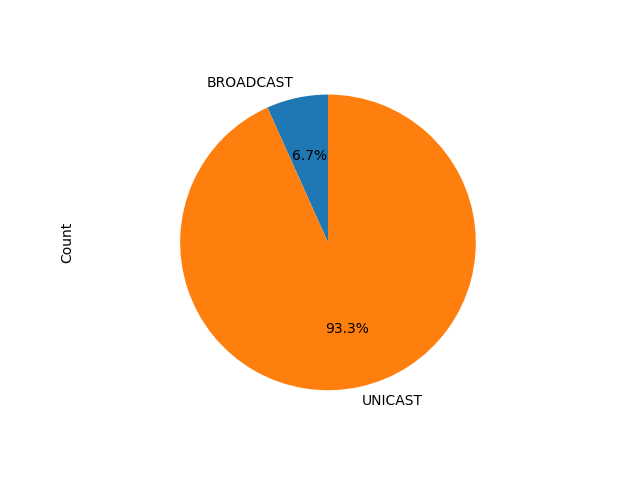
\includegraphics[width=8.5cm]{figs/broadcast_proportion_hogar_ethernet_S1_output.png}
 \caption{\normalfont Proporción de paquetes unicast/broadcast en la captura}
\end{figure}

Como se puede ver en el siguiente diagrama de torta los protocolos encontrados fueron $ARP$ e $IP$ (tanto v4 como v6), el protocolo de internet utilizado para transmitir mensajes, por ejemplo datos de usuarios, entre redes LAN.

\begin{figure}[H]
 \centering
 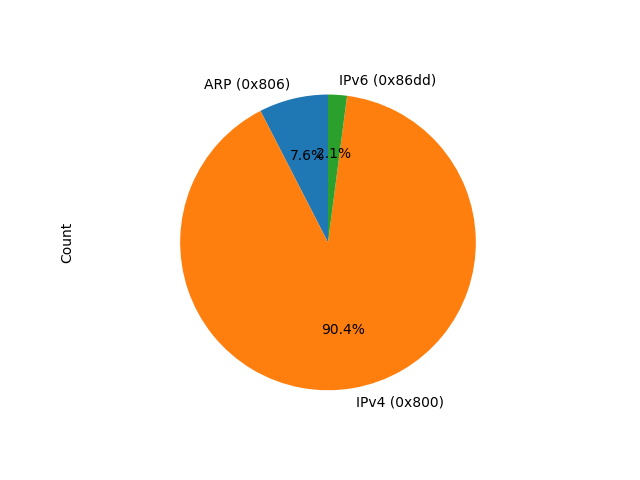
\includegraphics[width=8.5cm]{figs/protocols_proportion_hogar_ethernet_S1_output.png}
 \caption{\normalfont Proporción de protocolos en la captura}
\end{figure}

Habiendo visto el primer gráfico de torta no debería llamar la atención ver que el símbolo de menor entropía, o sea el más frecuente o de mayor probabilidad, es un unicast. En particular el protocolo con menor información es IPv4, lo que es consistente con ser el protocolo más popular en la red.

Debido a este símbolo destacado también sucede que la entropía no es máxima, aún cuando el resto de los símbolos tienen una distribución más uniforme entre sí.

\begin{figure}[H]
 \centering
 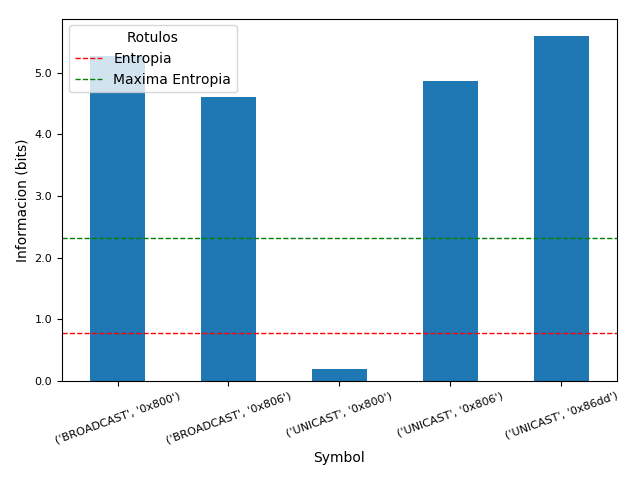
\includegraphics[width=8.5cm]{figs/information_hogar_ethernet_S1_output.png}
 \caption{\normalfont Información de los símbolos de la fuente S1, notando la entropía de la fuente, y la máxima entropía posible si la fuente fuera equiprobable.}
\end{figure}

\subsubsection*{Resultados fuente S2}

En el siguiente gráfico se pueden ver 4 hosts con baja entropía y 5 con alta entropía. Según nuestra hipótesis será de esperarse que el router sea uno de los primeros 4, idealmente el de menor entropía.

\begin{figure}[H]
 \centering
 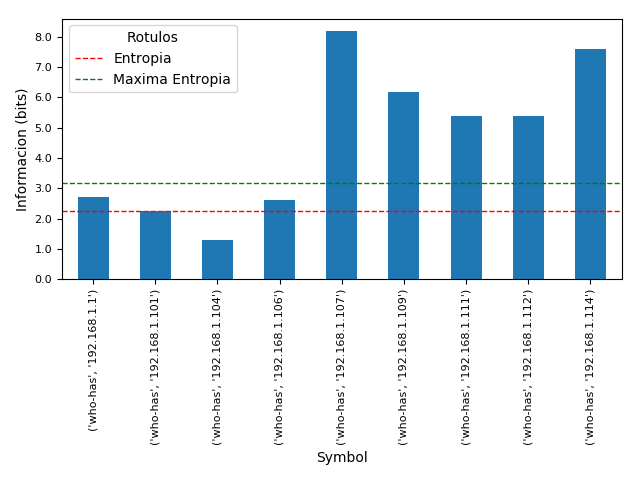
\includegraphics[width=8.5cm]{figs/information_hogar_ethernet_S2_output.png}
 \caption{\normalfont Información de los símbolos de la fuente S2, notando la entropía de la fuente, y la máxima entropía posible si la fuente fuera equiprobable.}
\end{figure}


A partir de los paquetes que se intercambian en la red armamos el grafo subyacente. En este cada vértice representa una IP local y cada arista va del origen al destino de un paquete who-has del protocolo ARP.

En este grafo los dos nodos con mayor grado son 192.168.1.1 y 192.168.1.112

\begin{figure}[H]
\centering
	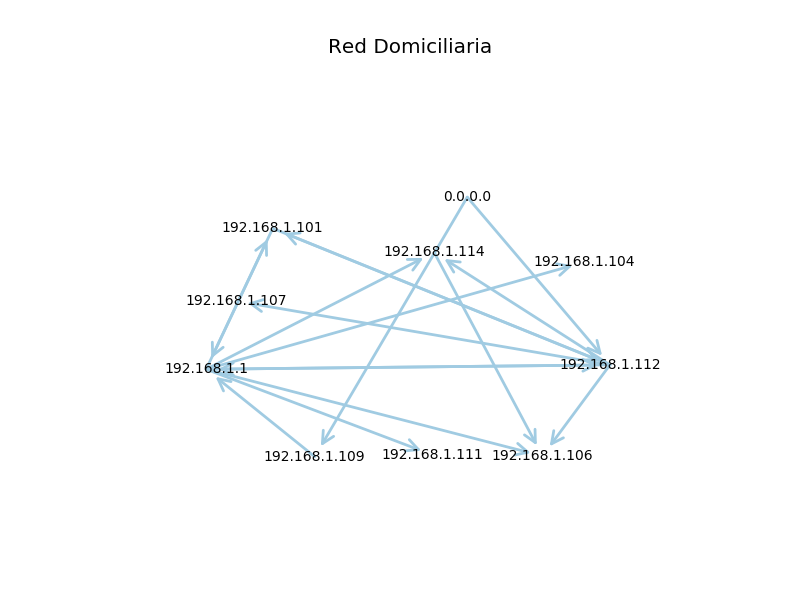
\includegraphics[width=8.5cm]{figs/grafo_red_domiciliaria.png}
	\caption{Grafo resultante de la red ethernet de una red domiciliaria durante la noche de un martes.}
	\label{fig:hogar-grafo}
\end{figure}

Cómo se puede ver si bien las dos técnicas utilizadas (Entropía y grafo subyacente) parecen apuntar a un conjunto pequeño de IPs no queda claro cuál sería el rol de cada IP o cual sería por ejemplo el router, el cual nosotros sabemos que es el 192.168.1.1, estos problemas probablemente se dan debido al tamaño de la red el cual no tiene una variedad suficientemente amplia de paquetes como para hacer robustas nuestras herramientas de predicción de símbolos destacados.

\subsection*{Red Oficina PyMe}
\subsubsection*{Resultados fuente S1}

Los paquetes broadcast representan casi el $25\%$ del total, esto es considerablemente más que en el caso anterior, una posible explicación es que la tabla de ARP de algún host se haya limpiado recientemente generando que este tenga que enviar varios who-is broadcast en la red.

\begin{figure}[H]
 \centering
 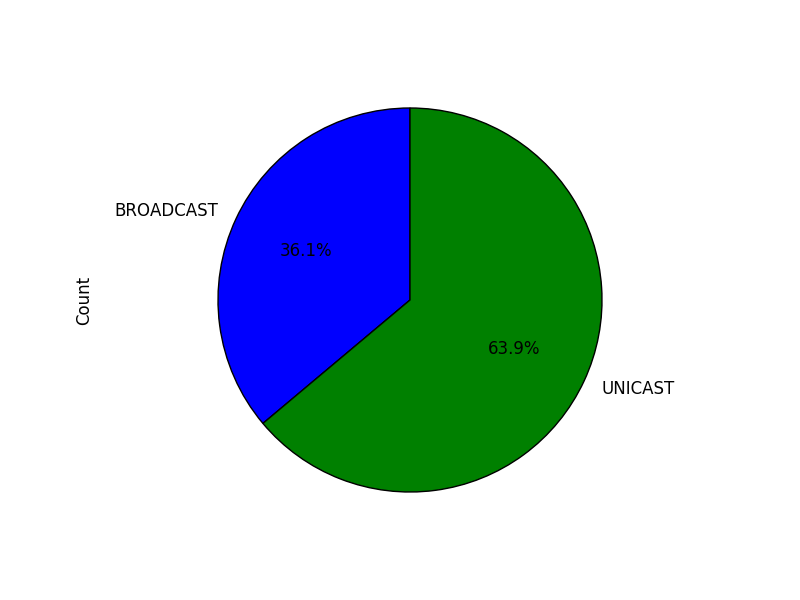
\includegraphics[width=8.5cm]{figs/broadcast_proportion_oficina_mediana_wifi_S1_output.png}
 \caption{\normalfont Proporción de paquetes unicast/broadcast en la captura}
\end{figure}

La cantidad de paquetes ARP es bastante alta apoyando la hipótesis dicha anteriormente sobre la gran cantidad de broadcasts.

\begin{figure}[H]
 \centering
 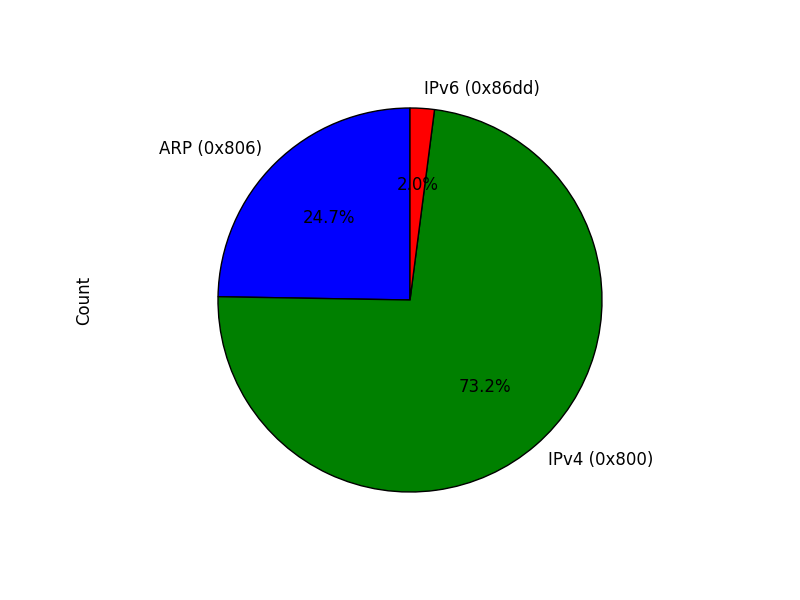
\includegraphics[width=8.5cm]{figs/protocols_proportion_oficina_mediana_wifi_S1_output.png}
 \caption{\normalfont Proporción de protocolos en la captura}
\end{figure}

El resultado es similar al visto en la red anterior dando como símbolo destacado un $(unicast, IPv4)$.

\begin{figure}[H]
 \centering
 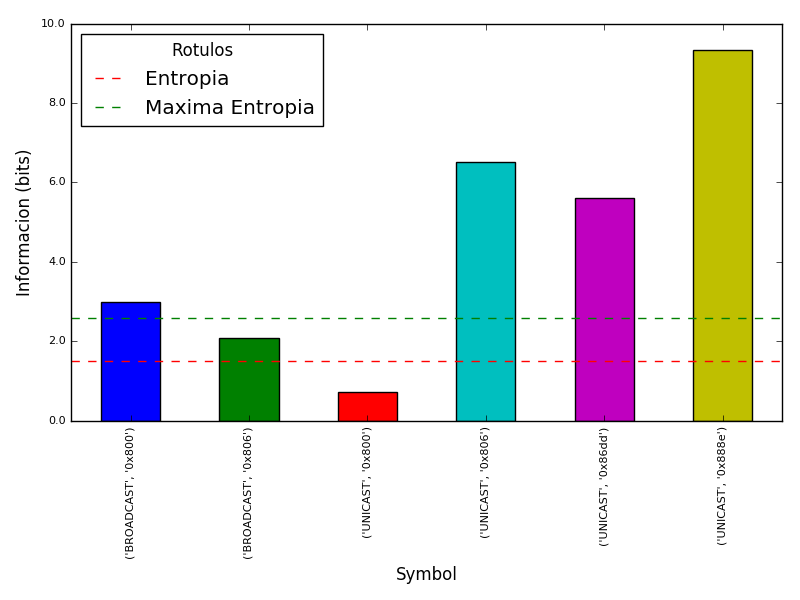
\includegraphics[width=8.5cm]{figs/information_oficina_mediana_wifi_S1_output.png}
 \caption{\normalfont Información de los símbolos de la fuente S1, notando la entropía de la fuente, y la máxima entropía posible si la fuente fuera equiprobable.}
\end{figure}

\subsubsection*{Resultados fuente S2}

En esta red hay un claro símbolo destacado con una entropía significativamente menor que la de cualquier otro.

\begin{figure}[H]
 \centering
 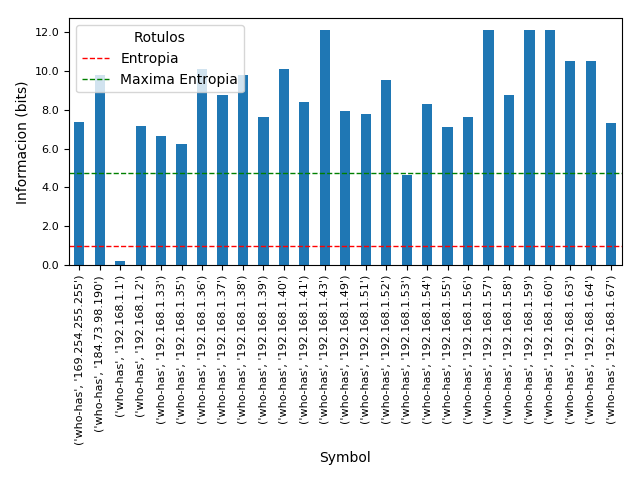
\includegraphics[width=8.5cm]{figs/information_oficina_mediana_wifi_S2_output.png}
 \caption{\normalfont Información de los símbolos de la fuente S2, notando la entropía de la fuente, y la máxima entropía posible si la fuente fuera equiprobable.}
\end{figure}

Utilizando el grafo subyacente para corroborar lo visto podemos ver que efectivamente el host 192.168.1.1 destaca (En el grafo tiene un grado mucho más alto que los demás nodos).

\begin{figure}[H]
\centering
 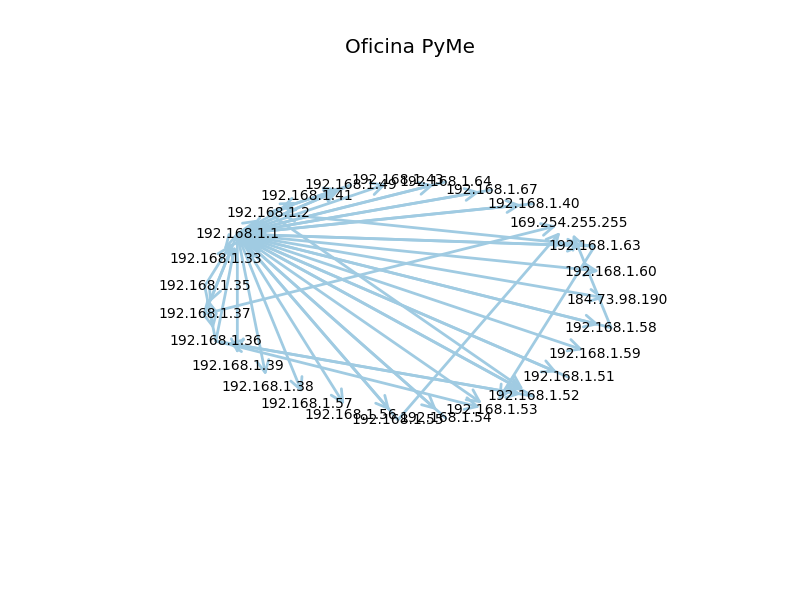
\includegraphics[width=8.5cm]{figs/grafo_pyme.png}
 \caption{Grafo resultante de la red wifi de una red pública en un starbucks durante la tarde de un día de semana.}
 \label{fig:domicilio-grafo}
\end{figure}

A diferencia del experimento con la red hogareña pudimos detectar correctamente el router de la red, esto apoya nuestra hipótesis de que el método estadístico funciona mejor con redes más grandes.

\subsection*{Red laboratorios}


\subsubsection*{Resultados fuente S1}

Al igual que con la primer red, los paquetes broadcast comprenden aproximadamente el $5\%$.

\begin{figure}[H]
 \centering
 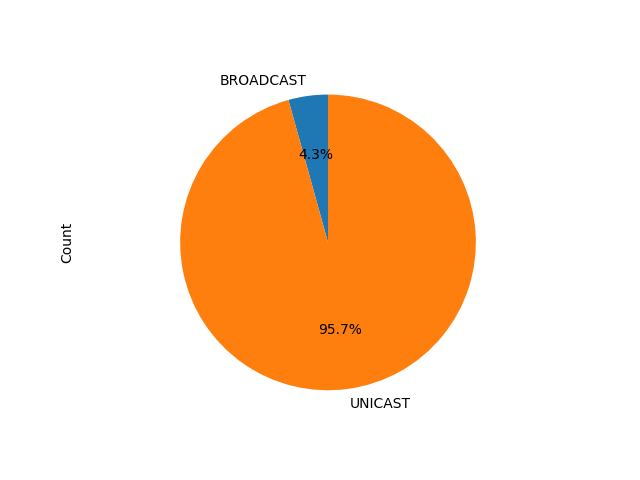
\includegraphics[width=8.5cm]{figs/broadcast_proportion_labo6_2018_04_18_S1_output.png}
 \caption{\normalfont Proporción de paquetes unicast/broadcast en la captura}
\end{figure}

Los paquetes ARP comprenden menos del $5\%$ lo cual parece indicar que la red está bastante estable. También hay algunos pocos paquetes IPv6, confirmando su escasez en comparación al protocolo IPv4.

\begin{figure}[H]
 \centering
 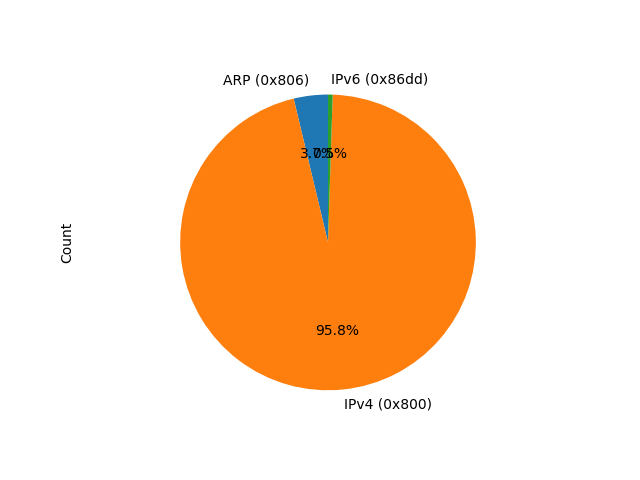
\includegraphics[width=8.5cm]{figs/protocols_proportion_labo6_2018_04_18_S1_output.png}
 \caption{\normalfont Proporción de protocolos en la captura}
\end{figure}

Al igual que en los casos anteriores el símbolo de menor entropía es un unicast de protocolo IPv4 (0x800), es interesante observar como dependiendo del protocolo varía si unicast o broadcast tiene mayor información. Por ejemplo con el protocolo ARP (0x806), los broadcasts tienen menor cantidad de bits, contrariamente a lo que pasa con IPv4. Esta tendencia se vió en todos los casos.

\begin{figure}[H]
 \centering
 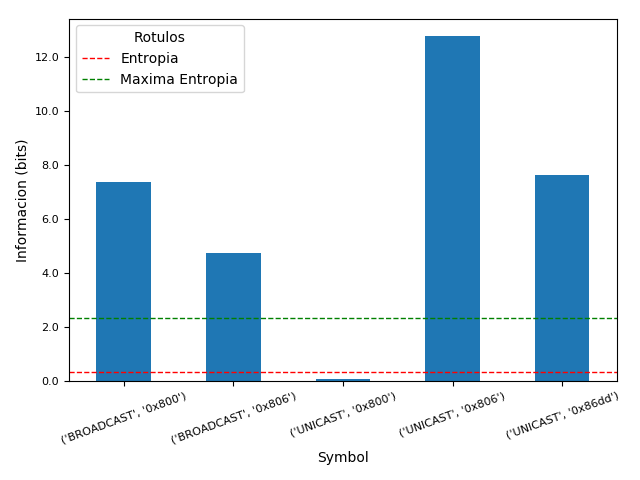
\includegraphics[width=8.5cm]{figs/information_labo6_2018_04_18_S1_output.png}
 \caption{\normalfont Información de los símbolos de la fuente S1, notando la entropía de la fuente, y la máxima entropía posible si la fuente fuera equiprobable.}
\end{figure}

\subsubsection*{Resultados fuente S2}

Destaca completamente el símbolo 10.2.203.254, este parece ser un destino muy frecuente de los paquetes who-has.

\begin{figure}[H]
 \centering
 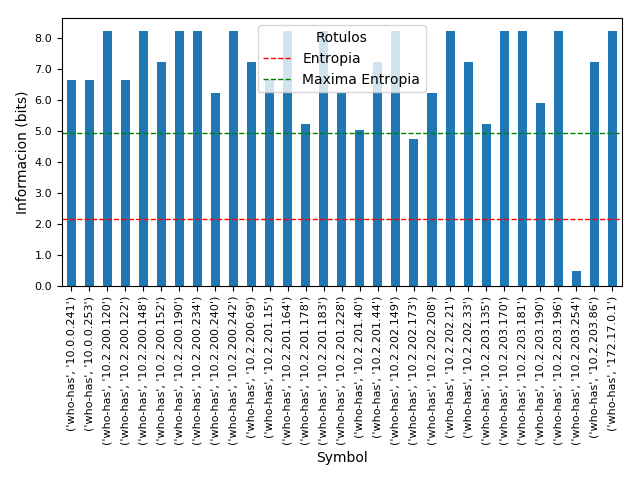
\includegraphics[width=8.5cm]{figs/information_labo6_2018_04_18_S2_output.png}
 \caption{\normalfont Información de los símbolos de la fuente S2, notando la entropía de la fuente, y la máxima entropía posible si la fuente fuera equiprobable.}
\end{figure}

En este grafo, el cual es mucho más grande que los anteriores, el nodo 10.2.203.254 es el de mayor grado corroborando lo visto en el gráfico de entropía.

\begin{figure}[H]
\centering
	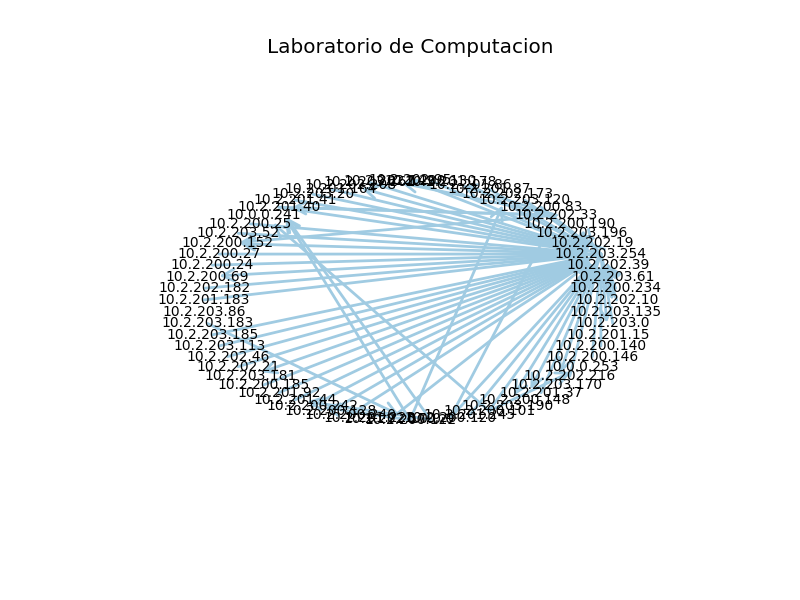
\includegraphics[width=8.5cm]{figs/grafo_dc.png}
	\caption{Grafo resultante de la red wifi del laboratorio de computación de la facultad a las 18 PM de un miércoles.}
	\label{fig:dc-grafo}
\end{figure}

De nuevo volvemos a detectar al router gracias a nuestra técnica de buscar al símbolo de menor entropía, esta parece funcionar muy bien en redes de gran tamaño.